\documentclass[12pt]{report}
\usepackage[utf8]{inputenc}
\usepackage{algpseudocode}
\usepackage[italian]{babel}
\usepackage{amsfonts}
\usepackage{amsmath}
\usepackage{subfig}
\usepackage{graphicx}
\usepackage{listings}
\usepackage{newtxtt}
\usepackage{hyperref}
\graphicspath{ {./pic/} }

\lstset{language=SQL}
\lstset{basicstyle=\ttfamily, keywordstyle=\bfseries}
\usepackage[utf8]{inputenc}

\title{\textbf{Gestione impianto produttivo e logistico per Babbo Natale}\\ [1ex] \large \textbf{Progetto per l'insegnamento di Basi di dati 90107}}
\author{Gabriele Crestanello \\\#970352 \\ gabriele.crestanello@studio.unibo.it\\ \\
Mattia Girolimetto\\ \#977478\\ mattia.girolimetto@studio.unibo.it}
\date{Dicembre 2022}

\begin{document}
\maketitle
\tableofcontents
\chapter{Analisi dei requisiti}
\section{Prima intervista}
\subsection{Requisiti iniziali}

Babbo Natale vuole digitalizzare la sua impresa e chiede il nostro aiuto per la
progettazione della base di dati. 

Per consegnare i regali in tutto il mondo Babbo ha assunto dei "babbi delegati"
ed ha assegnato a ciascuno di loro un paese di competenza, una slitta e relative
renne per fare le consegne. Ad ogni bambino della "lista dei bimbi buoni" si 
consegnano uno o più regali. Ciascun regalo viene prodotto interamente ed 
esclusivamente da un solo elfo manifatturiero. Di questi si vuole tenere traccia 
dei dati personali e contrattuali (es. nome, cognome, stipendio, ...) e a quali 
regali è stato assegnato. 
Si vuole inoltre tenere traccia del processo di costruzione di ciascun regalo
(da fare, in costruzione o fatto). Per costruire un regalo sono necessari 
dei materiali (legno, ferro, chiodi, ...), acquistati ciascuno da un fornitore
fidato. Per conservare i materiali sono adibiti vari magazzini, ciascuno dei
quali è destinato ad una o più categorie di materiali (es il magazzino 1 ha 
legno e chiodi, il magazzino 2 ha ferro e polistirolo e colla...). Si vuole 
sapere in ogni momento la quantità di materiale rimasto.
L'impianto produttivo è diviso in officine, ciascuna identificata da un 
codice univoco formato da una lettera e un numero (es "A13", "D7", ...) il cui
significato è noto solo a Babbo Natale. In ciascuna officina lavora un numero
arbitrario di elfi e ciascun elfo lavora in una sola officina.

\subsection{Operazioni richieste}
\begin{enumerate}
    \item Dati nome e cognome di un bambino, restituire i nomi e cognomi dei babbi delegati 
    che gli hanno consegnato i regali.
    \item Restituire nome e cognome di tutti gli elfi che hanno prodotto almeno un regalo
    trasportato da un dato babbo delegato.
    \item Restituire il costo per produrre un dato regalo. 
    \item Ricostruire l'albero genialogico di una data renna.
    \item Restituire nomi e cognomi dei bambini presenti nella lista dei bambini correntemente buoni.
    \item Trovare nomi e cognomi di tutti i bambini che in passato erano buoni e che correntemente non
    lo sono più.
    \item Restituire lo stock rimanente dei materiali necessari per la
    costruzione dei regali destinati a bambini italiani.
    \item Dato un elfo, restituire l’elenco di tutti i materiali (ordinati
    per categoria) che ha usato per la costruzione di regali nel corso del tempo.
    \item Restituire nomi e cognomi dei bambini che hanno ricevuto
    una consegna da un determinato modello di slitta nel corso del tempo.
    \item Restituire nome, cognome e orario di lavoro di tutti gli elfi
    attualmente in attività.
    \item Restituire i fornitori ordinati in base al valore dei materiali
    venduti e attualmente in magazzino.
    \item Data una renna restituire tutti i suoi fratelli e sorelle.
    \item Restituire la somma di tutti gli stipendi che babbo natale
    paga ai suoi dipendenti.
\end{enumerate}


\section{Ulteriori interviste}
Sono state poste ulteriori domande al cliente per ottenere ulteriori dettagli e
risolvere alcune ambiguità. Sono riporate sottostante le conclusioni:
\begin{itemize}
  \item Ogni categoria di materiale è contenuta \textit{esclusivamente} in un
    singolo magazzino.
  \item Le slitte, quando non in uso, vengono parcheggiate in dei garage.
  \item Garage e magazzini sono identificati da un codice univoco come quello
    usato per le officine.
  \item Questo codice univoco è in forma 
  \begin{center}$[A-Z][0-9][0-9]?$\end{center} ovvero
    una lettera seguita da una o due cifre.
  \item Le officine e i magazzini hanno degli orari di apertura e chiusura. Non è
    quindi sempre possibile accedere a questi edifici.
  \item Essendo le renne allevate dal personale di Babbo Natale 
    si vuole tenere traccia anche del loro albero genialogico, nonché della 
    loro nascita ed eventuale morte.
  \item La lista dei bimbi buoni viene aggiornata ogni anno. Se un bimbo è stato
    buono nel 2022 potrebbe non esserlo nel 2023, e viceversa.
  \item Quando un babbo delegato viene assunto riceve in affidamento una slitta
    che userà fino alla scadenza del suo contratto.
  \item Ogni babbo delegato ha un solo stato di competenza, ma più babbi delegati
    potrebbero avere assegnato lo stesso stato. Questo per poter consegnare i regali
    in modo efficente anche in paesi la popolazione è molto numerosa. 
\end{itemize}

A seguito di questa seconda intervista i requisiti non contengono più ambiguità.

\section{Glossario dei termini}
\begin{tabular}{|p{0.33\textwidth}|p{0.33\textwidth}|p{0.33\textwidth}|}
\hline
\textbf{Termine} & \textbf{Significato} & \textbf{Sinonimi} \\
\hline
Babbo delegato & Persona assunta da Babbo Natale per fare le consegne & Delegato \\
\hline
Elfo Manifatturiero & Entità assunta da Babbo Natale per costruire i regali & Elfo \\
\hline
Bambino Buono & Bambino il cui nome è nella lista dei bimbi buoni di Babbo Natale & Bambino \\
\hline
Conesegna & Insieme di regali destinati ad uno stesso bambino buono & - \\
\hline
Magazzino & Edificio in cui si conservano materiali & - \\
\hline
Officina & Edificio in cui gli elfi costruiscono i regali & - \\
\hline
Garage & Edificio in cui vengono conservate le slitte & - \\
\hline
Codice Univoco & Stringa alfanumerica nel formato

$[A-Z][0-9][0-9]?$ & - \\
\hline
\end{tabular}

\chapter{Progettazione}
\section{Progettazione concettuale}
\subsection{Identificare entità, relazioni e attributi}
Dopo aver studiato attentamente i requisiti sono state ricavate delle 
proposizioni utili per identificare entità, relazioni e attributi. Di seguito
queste sono elencate affiancate alla loro rappresentazione secondo il modello
entità-relazione.

\paragraph{Proposizioni sui Babbi delegati}
\begin{itemize}
  \item Esistono dei babbi delegati
  \item Esistono degli stati
  \item Ogni delegato ha uno e uno solo stato di competenza
  \item Esistono delle slitte
  \item Ogni delegato ha una sola slitta, che userà per tutta la durata del suo contratto
\end{itemize}
\begin{center}
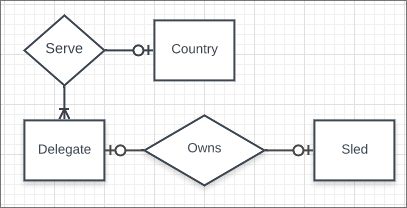
\includegraphics[scale=0.60]{er1.png}
\end{center}

\paragraph{Proposizioni su slitte e renne}
\begin{itemize}
  \item Esistono dei garage
  \item Le slitte vengono parcheggiate nei garage
  \item Esistono delle renne
  \item Ogni renna ha una madre, un padre, una data di nascita e eventualmente di morte
  \item Ogni slitta ha delle renne
  \item Ogni garage ha un codice univoco
\end{itemize}
\begin{center}
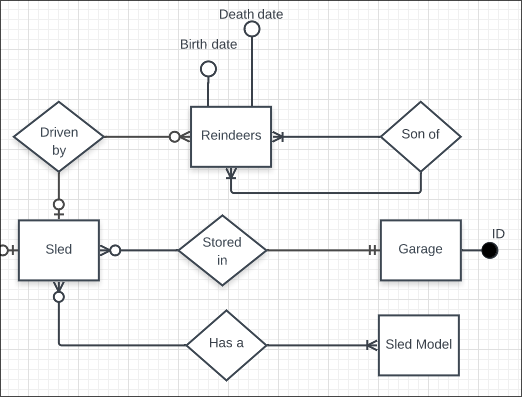
\includegraphics[scale=0.60]{er2.png}
\end{center}

\paragraph{Proposizioni su bambini e regali}
\begin{itemize}
  \item Esistono dei bambini
  \item Ogni bambino può essere buono o no
  \item Esistono dei regali
  \item Ogni bambino buono ha diritto ad uno o più regali
\end{itemize}
\begin{center}
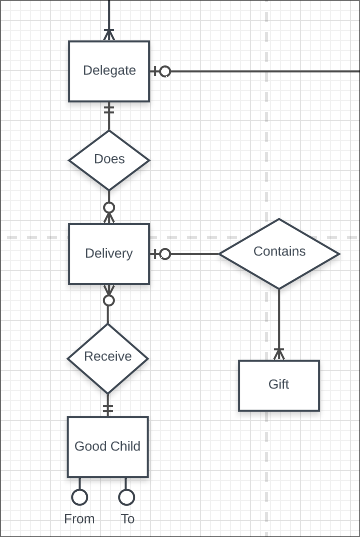
\includegraphics[scale=0.60]{er3.png}
\end{center}

\paragraph{Proposizioni su elfi e materiali}
\begin{itemize}
  \item Esistono degli elfi
  \item Ogni regalo è prodotto da un singolo elfo
  \item Ogni elfo ha dei dati personali e contrattuali
  \item Ogni regalo ha uno stato di costruzione
  \item Esistono dei materiali
  \item Ogni regalo è costruito con dei materiali
\end{itemize}
\begin{center}
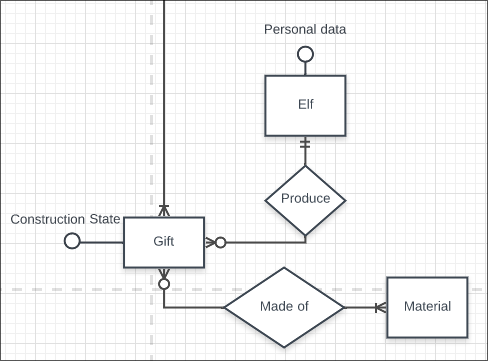
\includegraphics[scale=0.60]{er4.png}
\end{center}

\paragraph{Proposizioni su categorie di materiali e fornitori}
\begin{itemize}
  \item Esistono dei fornitori
  \item Esistono delle categorie di materiali
  \item Ogni materiale ha una categoria
  \item Ogni categoria di materiali è acquistata da un fornitore
  \item Ogni fornitore ci vende una o più categorie
  \item Esistono dei magazzini
  \item Ogni magazzino ha un codice univoco
  \item Ogni magazzino ha delle categorie di meriali
\end{itemize}
\begin{center}
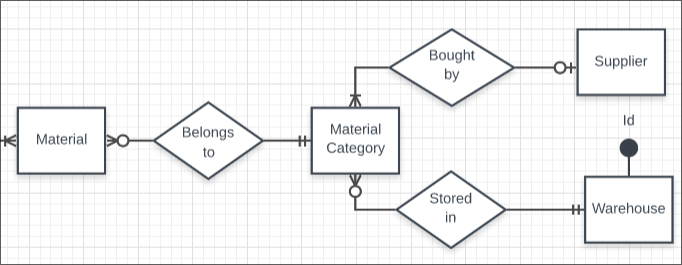
\includegraphics[scale=0.50]{er5.png}
\end{center}

\paragraph{Proposizioni sulle officine}
\begin{itemize}
  \item Esistono delle officine
  \item Ogni officina ha un codice univoco
  \item Ogni elfo lavora in un'officina
  \item Ogni officina ha degli elfi che ci lavorano dentro
\end{itemize}
\begin{center}
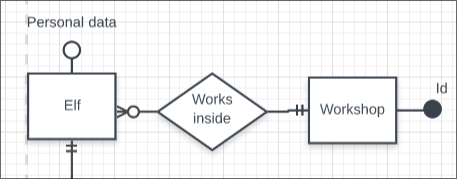
\includegraphics[scale=0.70]{er6.png}
\end{center}

\subsection{Gerarchie IS-A}
Usando questa modellazione dei dati sono state individuate due possibili 
gerarchie \textit{is-a}.

\paragraph{Impiegati}
La prima riguarda le entità \textit{Elfo} e \textit{Delegato}. Queste infatti
rappresentano due tipologie di impieghi all'interno dell'azienda di Babbo Natale.
Per questo possono essere viste come una specializzazione di un'entità generale
\textit{Impiegato}, che avrà come attributi, ad esempio, tutte le informazioni 
del contratto di assunzione.
\begin{center}
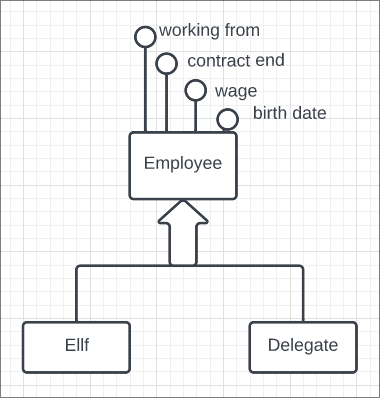
\includegraphics[scale=0.50]{isa1.png}
\end{center}

\paragraph{Edifici}
La seconda realazione \textit{is-a} individuata è quella tra le entità che rappresentano 
gli edifici, ovvero \textit{garage}, \textit{workshop} e \textit{warehouse}. Questi infatti
condividono informazioni comuni come l'indirizzo e il codice univoco (nello stesso formato 
per tutti e tre). Analizzando più attentamente il problema si nota che \textit{workshop} e 
\textit{warehouse}, a differenza di \textit{garage}, condividono delle informazioni aggiuntive:
quelle riguardanti l'orario di apertura e chiusura dell'edificio. Quindi è stata individuata
una doppia relazione \textit{is-a}:
\begin{center}
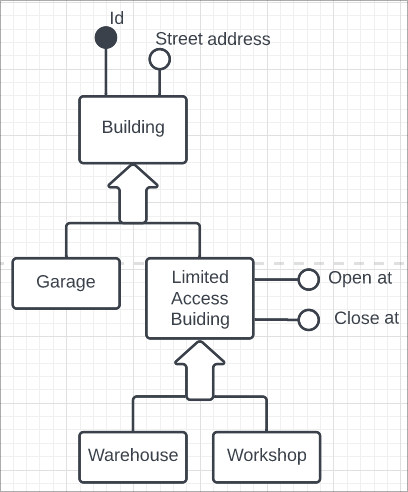
\includegraphics[scale=0.50]{isa2.png}
\end{center}

\subsection{Relazione ricorsiva}
Un' altra osservazione fatta riguarda la relazione ricorsiva \textit{son of} delle entità \textit{reindeers}.
Al fine di mantenere una più accurata rappresentazione della realtà e semplificare lo schema, è possibile
rimovere la relazione \textit{son of} di tipo \textit{molti a molti} ed inserire due relazioni di tipo
\textit{uno a molti}. Queste rappresentano il concetto di parentela madre-figlio e padre-figlio. Lo schema
diventa quindi:
\begin{center}
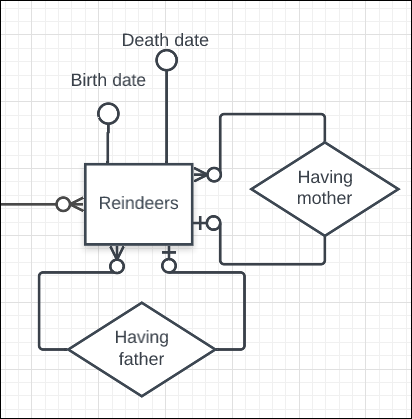
\includegraphics[scale=0.50]{ric1.png}
\end{center}

Si noti che sono state modificate anche le molteplicità: sebbene è impossibile per natura che una renna non abbia una
madre e un padre, si è preferito tenere la relazione opzionale nel caso in cui ci siano renne i cui genitori siano
sconosciuti. Nell'altro verso è stata scelta la molteplicità \textit{zero o molti} poiché è ragionevole pensare che una
renna possa non avere  figli.

\subsection{Conclusioni}
Alla fine della progettazione concettuale lo schema entità per intero è il seguente:

\begin{center}
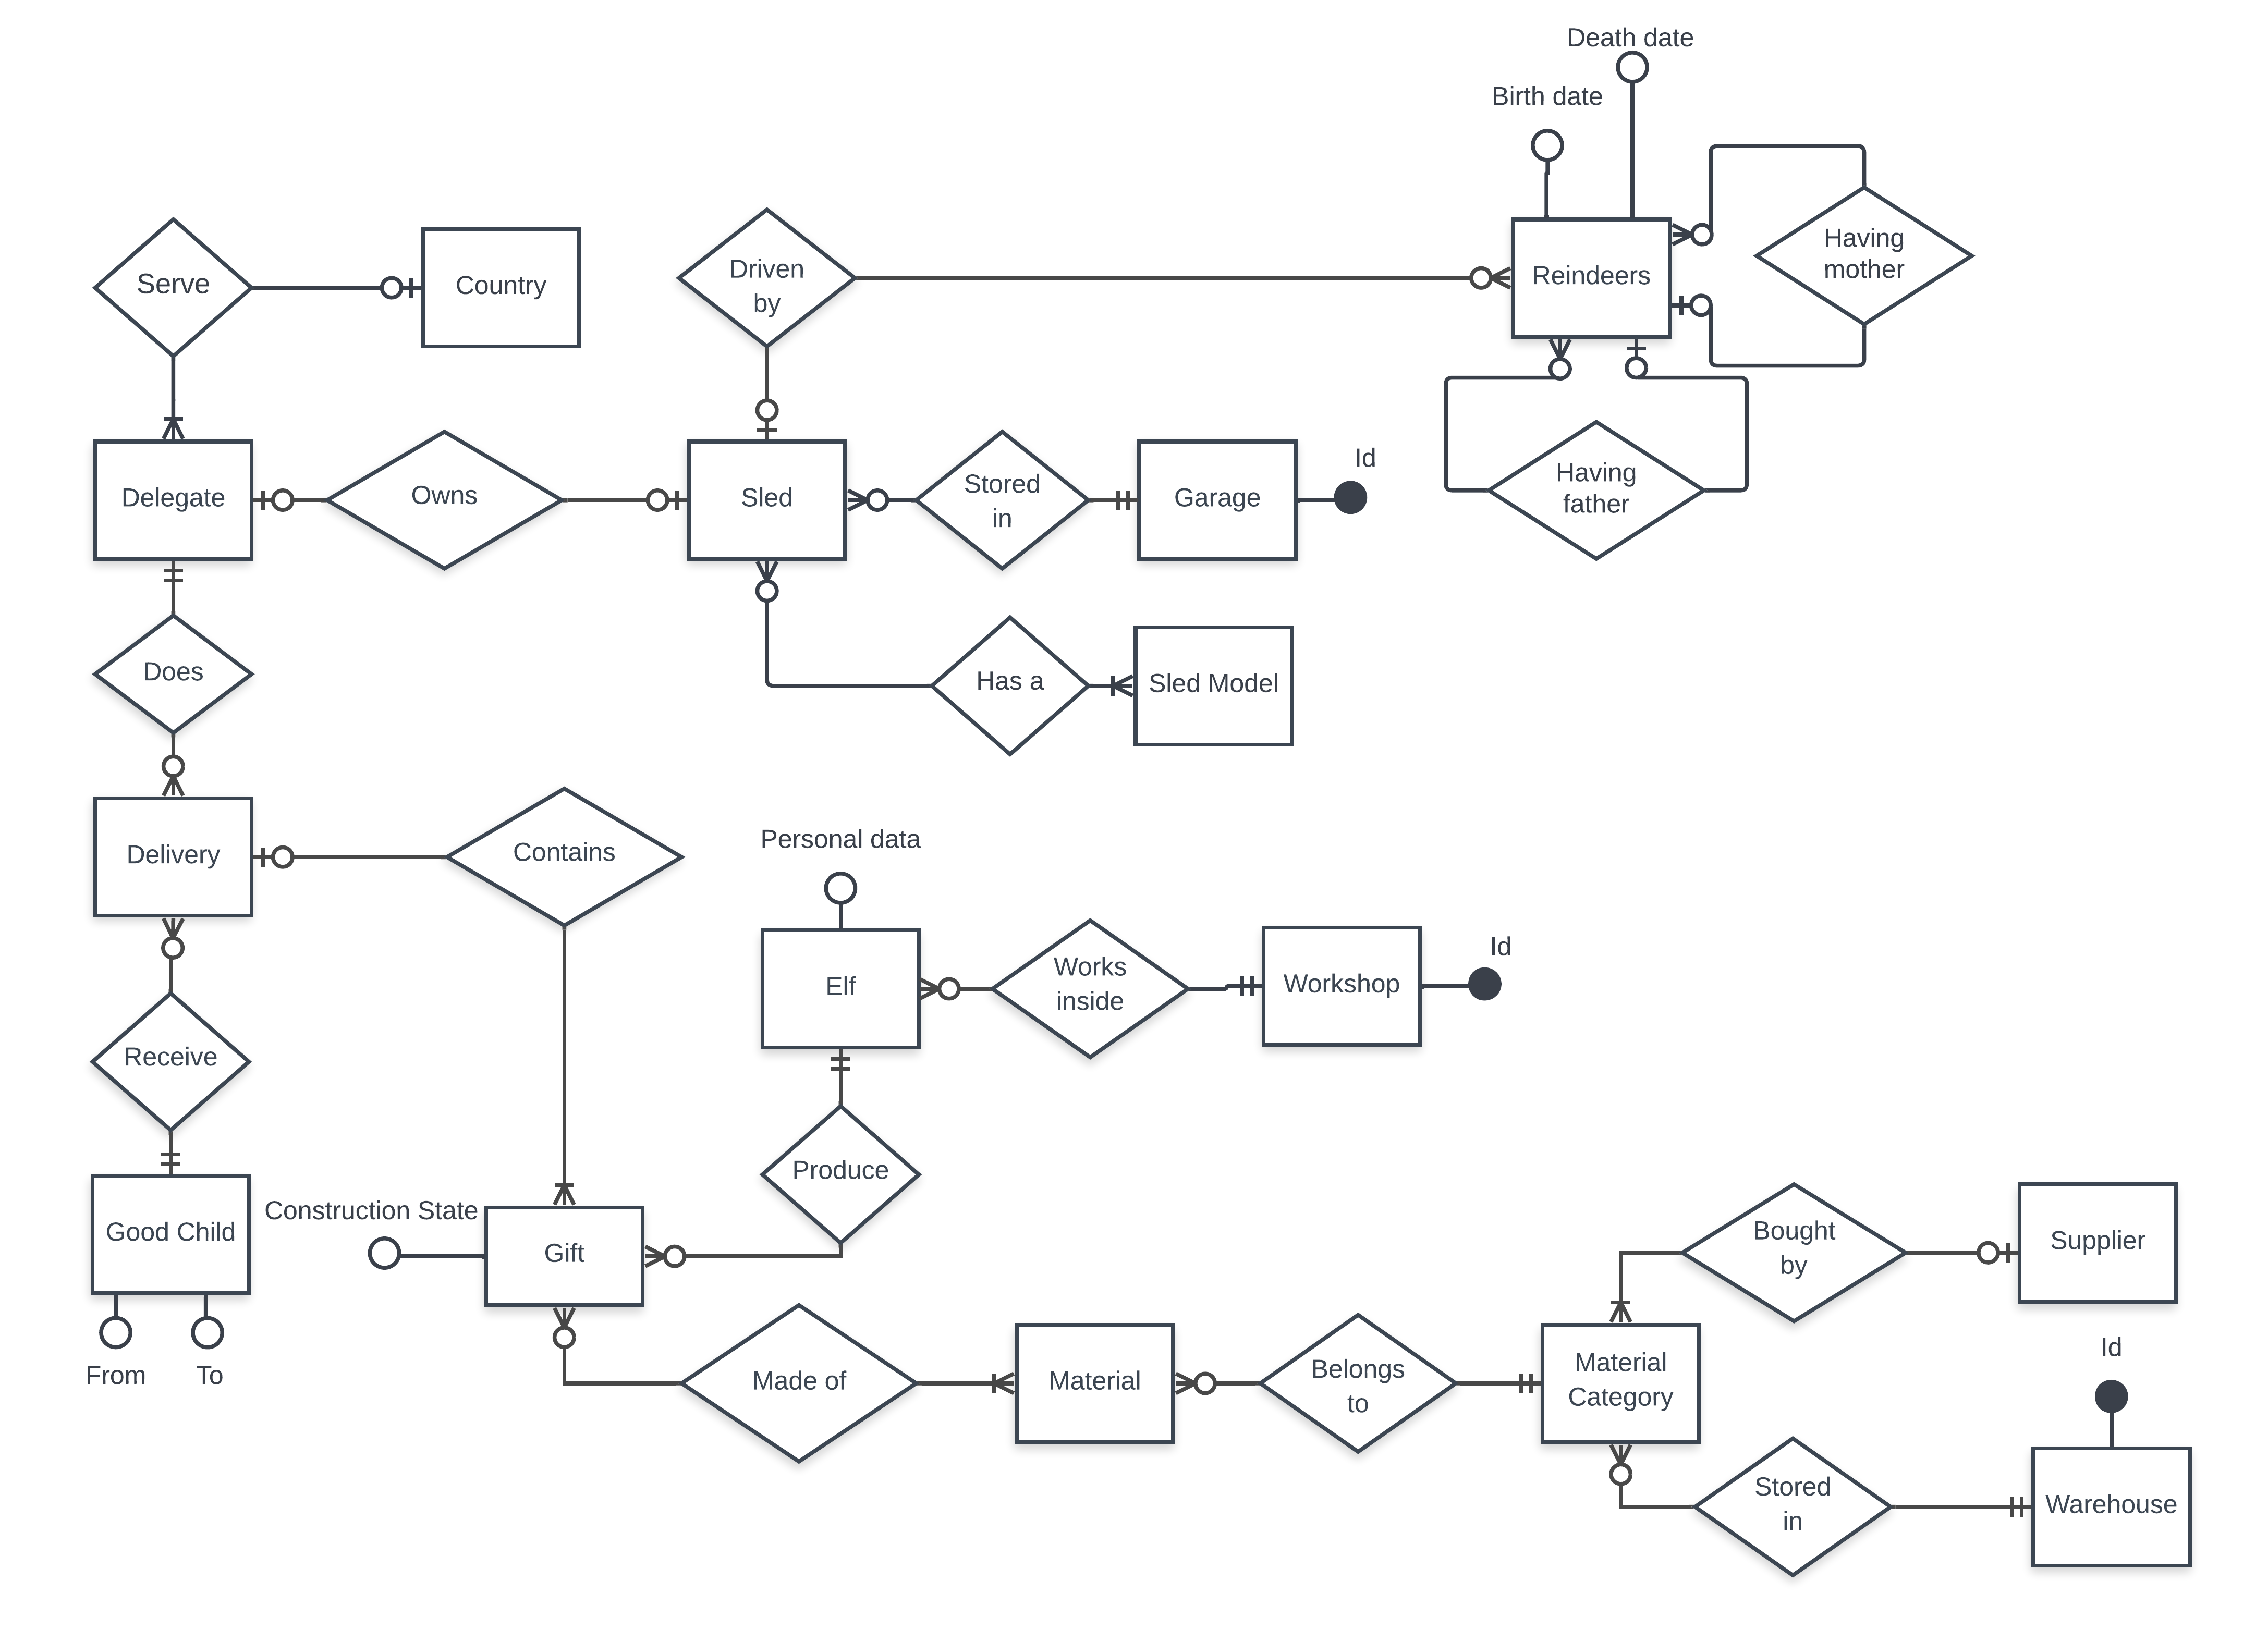
\includegraphics[width=1.3\linewidth]{ErComplete.png}
\end{center}
\section{Progettazione logica}

\subsection{Relazioni molti a molti}
Nello schema ER è presente una relazione di tipo \textit{molti a molti} tra le entità \textit{gift} e
\textit{material}. Per rappresentarla correttamente nel modello logico è stata aggiunta l'entità intermedia 
\textit{GiftMaterial} come segue

\begin{center}
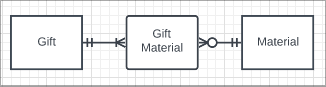
\includegraphics[scale=0.7]{m2m.png}
\end{center}

\subsection{Il caso dei bambini buoni}
Nello schema ER progettato i bambini buoni sono rappresentati da un'entità \textit{Good 
child} con campi \textit{from} e \textit{to}. Questi servono a dire che il bambino identificato dagli
attributi di quel elemento della relazione è \textit{stato buono da <from> a <to>}, dove $<to>$ può
assumere valore $NULL$ nel caso in cui il bimbo sia correntemente buono. Questo però implica una notevole
forma di ridondanza, in quanto per ogni cambiamento di stato di comportamento del bambino, si deve 
inserire un nuovo record nella tabella. Per risolvere questa ridondanza si è sostituita l'entità
\textit{GoodChild} con \textit{Child} e \textit{PeriodOfGoodness} come riportato in seguito:
\begin{center}
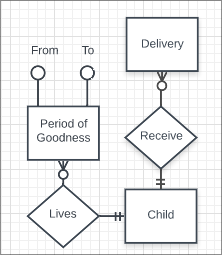
\includegraphics[scale=0.7]{goodChild.png}
\end{center}

\subsection{Tavole dei volumi e delle operazioni}
Sottostante sono riportate le tavole dei volumi e delle operazioni. Si noti che alcune tabelle (regali,
spedizioni ad esempio) tendono a crescere parecchio, in modo lineare, col passare degli anni.

\paragraph{Tabella dei volumi}
\begin{center}
\begin{tabular}{|p{0.40\textwidth}|p{0.10\textwidth}|p{0.20\textwidth}|}
\hline
\textbf{Concetto} & \textbf{Tipo} & \textbf{Volume} \\
\hline
Stato & E & 200 \\
\hline
Babbi Delegati & E & 400 \\
\hline
Slitte & E & 450 \\
\hline
Modelli di slitta & E & 50 \\
\hline
Garage & E & 20 \\
\hline
Renne & E & 2700 \\
\hline
Spedizioni & E & 2.200.000.000 \\
\hline
Bambini & E & 2.200.000.000 \\
\hline
Periodi di bontà & E & 2.200.000.000 \\
\hline
Regali & E & 6.600.000.000 \\
\hline
Elfi Manifatturieri & E & 500.000 \\
\hline
Officine & E & 1000 \\
\hline
Materiali & E & 5000 \\
\hline
Categorie di materiali & E & 500 \\
\hline
Fornitori & E & 500 \\
\hline
Magazzini & E & 100 \\
\hline
\end{tabular}
\end{center}

\paragraph{Tabella delle operazioni}
\begin{center}
\begin{tabular}{|p{0.40\textwidth}|p{0.40\textwidth}|}
\hline
\textbf{Operazione} & \textbf{Frequenza annuale} \\
\hline
1 & 1000 \\
\hline
2 & 1000 \\
\hline
3 & 7.000.000.000 \\
\hline
4 & 2700 \\
\hline
5 & 500 \\
\hline
6 & 500 \\
\hline
7 & 500 \\
\hline
8 & 1000 \\
\hline
9 & 500 \\
\hline
10 & 1000 \\
\hline
11 & 1000 \\
\hline
12 & 100 \\
\hline
13 & 2000 \\
\hline
\end{tabular}
\end{center}


\subsection{Schema logico}

\begin{tabular}{|p{0.25\textwidth}|p{0.40\textwidth}|p{0.35\textwidth}|}
\hline
\textbf{Entità} & \textbf{Attributi} & \textbf{Relazioni} \\
\hline
Country & \underline{Id}, Name, SurfaceArea & \\
\hline
Delegate & \underline{Id}, Name, Surname, Wage, WorkingFrom, WorkingTo, BirthDate, CountryId, SledId & CountryId $\rightarrow$ Country.Id

SledId $\rightarrow$ Sled.Id \\ 
\hline
Sled & \underline{Id}, GarageId, ModelId, BuyDate & \\
\hline
SledModel & \underline{Id}, manufacturer, code &   \\ 
\hline
Garage & \underline{Id}, StreetAddress, Slots &  \\
\hline
Reindeer & \underline{Id}, SledId, Name, BirthDate, DeathDate, FatherId, MotherId & SledId $\rightarrow$ Sled.Id

FatherId $\rightarrow$ Reindeer.Id

MotherId $\rightarrow$ Reindeer.Id \\
\hline
Delivery & \underline{Id}, LeavingTime, DeliveryTime, DelegateId, ChildId & DelegateId $\rightarrow$ Delegate.Id,

ChildId $\rightarrow$ Child.Id \\ 
\hline
Child & \underline{Id}, BirthDate, Name, Surname, StreetAddress, City, CountryId, ZIP & CountryId $\rightarrow$ 
Country.Id \\
\hline
PeriodOfGoodness & \underline{Id}, From, To , ChildId & ChildId $\rightarrow$ Child.Id \\
\hline
Gift & \underline{Id}, ConstructionState, DeliveryId, ElfId & DeliveryId $\rightarrow$ Delivery.Id

ElfId $\rightarrow$ Elf.Id \\
\hline
GiftMaterial & \underline{Id}, MaterialQuantity, UnitOfMeasurement, GiftId, MaterialId & GiftId $\rightarrow$ Gift.Id

MaterialId $\rightarrow$ Material.Id \\
\hline
Elf & \underline{Id}, Name, Surname, Wage, WorkingFrom, WorkingTo, BirthDate, WorkshopId & WorkshopId $\rightarrow$ Workshop.Id \\
\hline
Workshop & \underline{Id}, Name, StreetAddress, Capacity, OpenAt, CloseAt &  \\
\hline
Material & \underline{Id}, Name, Stock, CategoryId & CategoryId $\rightarrow$ MaterialCategory.Id \\ 
\hline
MaterialCategory & \underline{Id}, Name, WarehouseId, SupplierId & WarehouseId $\rightarrow$ Warehouse.Id

SupplierId $\rightarrow$ Supplier.Id \\
\hline
Supplier & \underline{Id}, CompanyName, StreetAddress, City, CountryId, ZIP, Phone, Email & CountryId $\rightarrow$ Country.Id \\
\hline
Warehouse & \underline{Id}, Name, StreetAddress, OpenAt, CloseAt, Capacity &  \\ 
\hline

\end{tabular}

\begin{center}
    \includegraphics[scale=0.35]{babbodb.png}
\end{center}

\subsection{Normalizzazione}
E' possibile dimostrare che lo schema logico rappresentato in precedenza è nella forma normale di Boyce-Codd.
Ciascuna relazione infatti presenta solo dipendenze funzionali non banali il cui determinante è una chiave o
una possibile super chiave.

\chapter{Codifica SQL}
\subsection{Definizione dello schema}

\begin{lstlisting}
CREATE type CONS_STATE AS ENUM (
    'to do',
    'designing',
    'sculpting',
    'crafting',
    'painting',
    'forging',
    'finished'
);


CREATE TABLE IF NOT EXISTS country (
        id SERIAL PRIMARY KEY,
        name VARCHAR(255) NOT NULL,
        surface_area INTEGER NOT NULL
    );

CREATE TABLE IF NOT EXISTS garage (
        id VARCHAR(3) PRIMARY KEY,
        street_address VARCHAR(255) NOT NULL,
        slots SMALLINT NOT NULL,
        created_at TIMESTAMP NOT NULL DEFAULT NOW(),
        updated_at TIMESTAMP NOT NULL DEFAULT NOW()
    );

CREATE TABLE IF NOT EXISTS sled_model (
        id SERIAL PRIMARY KEY,
        manufacturer VARCHAR(255) NOT NULL,
        code VARCHAR(255) NOT NULL UNIQUE
    );
CREATE TABLE IF NOT EXISTS sled (
        id SERIAL PRIMARY KEY,
        buy_date TIMESTAMP NOT NULL,
        garage_id VARCHAR(3) NOT NULL,
        model_id INTEGER NOT NULL,
        created_at TIMESTAMP NOT NULL DEFAULT NOW(),
        updated_at TIMESTAMP NOT NULL DEFAULT NOW(),
        FOREIGN KEY (garage_id) REFERENCES garage (id),
        FOREIGN KEY (model_id) REFERENCES sled_model (id)
    );

CREATE TABLE IF NOT EXISTS delegate (
        id SERIAL PRIMARY KEY,
        name VARCHAR(255) NOT NULL,
        surname VARCHAR(255) NOT NULL,
        wage REAL NOT NULL,
        working_from DATE NOT NULL DEFAULT NOW(),
        working_to DATE DEFAULT NULL,
        birth_date DATE NOT NULL,
        country_id INTEGER NOT NULL,
        sled_id INTEGER NOT NULL,
        created_at TIMESTAMP NOT NULL DEFAULT NOW(),
        updated_at TIMESTAMP NOT NULL DEFAULT NOW(),
        FOREIGN KEY (country_id) REFERENCES country (id),
        FOREIGN KEY (sled_id) REFERENCES sled (id),
        CHECK (working_from < working_to),
        CHECK (wage > 0)
    );
CREATE TABLE IF NOT EXISTS reindeer (
        id SERIAL PRIMARY KEY,
        name VARCHAR(255) NOT NULL,
        birth_date DATE NOT NULL,
        death_date DATE DEFAULT NULL,
        sled_id INTEGER NOT NULL,
        father_id INTEGER,
        mother_id INTEGER,
        created_at TIMESTAMP NOT NULL DEFAULT NOW(),
        updated_at TIMESTAMP NOT NULL DEFAULT NOW(),
        FOREIGN KEY (sled_id) REFERENCES sled (id),
        FOREIGN KEY (father_id) REFERENCES reindeer (id),
        FOREIGN KEY (mother_id) REFERENCES reindeer (id),
        CHECK(death_date > birth_date)
    );

CREATE TABLE IF NOT EXISTS child (
        id SERIAL PRIMARY KEY,
        name VARCHAR(255) NOT NULL,
        surname VARCHAR(255) NOT NULL,
        birth_date DATE NOT NULL,
        street VARCHAR(255) NOT NULL,
        city VARCHAR(255) NOT NULL,
        zip VARCHAR(255) NOT NULL,
        country_id INTEGER NOT NULL,
        created_at TIMESTAMP NOT NULL DEFAULT NOW(),
        updated_at TIMESTAMP NOT NULL DEFAULT NOW(),
        FOREIGN KEY (country_id) REFERENCES country (id)
    );
CREATE TABLE IF NOT EXISTS period_of_goodness (
        id SERIAL PRIMARY KEY,
        good_from SMALLINT NOT NULL,
        good_to SMALLINT DEFAULT NULL,
        child_id INTEGER NOT NULL,
        created_at TIMESTAMP NOT NULL DEFAULT NOW(),
        updated_at TIMESTAMP NOT NULL DEFAULT NOW(),
        FOREIGN KEY (child_id) REFERENCES child (id),
        CHECK (good_to > good_from)
    );

CREATE TABLE IF NOT EXISTS delivery (
        id SERIAL PRIMARY KEY,
        leaving_time TIMESTAMP DEFAULT NULL,
        delivery_time TIMESTAMP DEFAULT NULL,
        delegate_id INTEGER NOT NULL,
        child_id INTEGER NOT NULL,
        created_at TIMESTAMP NOT NULL DEFAULT NOW(),
        updated_at TIMESTAMP NOT NULL DEFAULT NOW(),
        FOREIGN KEY (delegate_id) REFERENCES delegate (id),
        FOREIGN KEY (child_id) REFERENCES child (id),
        CHECK (leaving_time < delivery_time)
    );

CREATE TABLE IF NOT EXISTS workshop (
        id VARCHAR(3) PRIMARY KEY,
        street_address VARCHAR(255) NOT NULL,
        capacity INTEGER NOT NULL DEFAULT 0,
        open_at TIME NOT NULL,
        close_at TIME NOT NULL,
        created_at TIMESTAMP NOT NULL DEFAULT NOW(),
        updated_at TIMESTAMP NOT NULL DEFAULT NOW(),
        CHECK (open_at < close_at)
    );
CREATE TABLE IF NOT EXISTS elf (
        id SERIAL PRIMARY KEY,
        name VARCHAR(255) NOT NULL,
        surname VARCHAR(255) NOT NULL,
        wage REAL NOT NULL,
        working_from DATE NOT NULL,
        working_to DATE DEFAULT NULL,
        birth_date DATE NOT NULL,
        workshop_id VARCHAR(3) NOT NULL,
        created_at TIMESTAMP NOT NULL DEFAULT NOW(),
        updated_at TIMESTAMP NOT NULL DEFAULT NOW(),
        FOREIGN KEY (workshop_id) REFERENCES workshop (id),
        CHECK (wage > 0),
        CHECK (working_from < working_to)
    );

CREATE TABLE IF NOT EXISTS gift (
        id SERIAL PRIMARY KEY,
        construction_state CONS_STATE NOT NULL,
        name VARCHAR(100) NOT NULL,
        delivery_id INTEGER NOT NULL,
        elf_id INTEGER NOT NULL,
        created_at TIMESTAMP NOT NULL DEFAULT NOW(),
        updated_at TIMESTAMP NOT NULL DEFAULT NOW(),
        FOREIGN KEY (delivery_id) REFERENCES delivery (id),
        FOREIGN KEY (elf_id) REFERENCES elf (id)
    );

CREATE TABLE IF NOT EXISTS warehouse (
        id VARCHAR(3) PRIMARY KEY,
        name VARCHAR(255) NOT NULL,
        streetAddress VARCHAR(255) NOT NULL,
        open_at TIME NOT NULL,
        close_at TIME NOT NULL,
        capacity INTEGER NOT NULL DEFAULT 0,
        created_at TIMESTAMP NOT NULL DEFAULT NOW(),
        updated_at TIMESTAMP NOT NULL DEFAULT NOW(),
        CHECK (open_at < close_at)
    );

CREATE TABLE IF NOT EXISTS supplier (
        id SERIAL PRIMARY KEY,
        company_name VARCHAR(255) NOT NULL,
        street VARCHAR(255) NOT NULL,
        city VARCHAR(255) NOT NULL,
        country_id INTEGER NOT NULL,
        zip VARCHAR(7) NOT NULL,
        phone VARCHAR(15) NOT NULL,
        email VARCHAR(255) NOT NULL,
        created_at TIMESTAMP NOT NULL DEFAULT NOW(),
        updated_at TIMESTAMP NOT NULL DEFAULT NOW(),
        FOREIGN KEY (country_id) REFERENCES country (id)
    );

CREATE TABLE IF NOT EXISTS material_category (
        id SERIAL PRIMARY KEY,
        name VARCHAR(255) NOT NULL,
        warehouse_id VARCHAR(3) NOT NULL,
        supplier_id INTEGER NOT NULL,
        FOREIGN KEY (warehouse_id) REFERENCES warehouse (id),
        FOREIGN KEY (supplier_id) REFERENCES supplier (id)
    );

CREATE TABLE IF NOT EXISTS material (
        id SERIAL PRIMARY KEY,
        name VARCHAR(255) NOT NULL,
        stock INTEGER NOT NULL DEFAULT 0,
        category_id INTEGER NOT NULL,
        unit_cost INTEGER NOT NULL,
        created_at TIMESTAMP NOT NULL DEFAULT NOW(),
        updated_at TIMESTAMP NOT NULL DEFAULT NOW(),
        FOREIGN KEY (category_id) REFERENCES material_category (id),
        CHECK (stock >= 0),
        CHECK (unit_cost >= 0)
    );

CREATE TABLE IF NOT EXISTS gift_material (
        id SERIAL PRIMARY KEY,
        material_quantity INTEGER NOT NULL DEFAULT 0,
        unit_of_measurement VARCHAR(64) NOT NULL,
        gift_id INTEGER NOT NULL,
        material_id INTEGER NOT NULL,
        FOREIGN KEY (gift_id) REFERENCES gift (id),
        FOREIGN KEY (material_id) REFERENCES material (id),
        CHECK (material_quantity > 0)
    );
\end{lstlisting}

\subsection{Definizione delle operazioni}

\paragraph{Operazione 1} Dati nome e cognome di un bambino, restituire i nomi e cognomi dei babbi delegati 
    che gli hanno consegnato i regali.
\begin{lstlisting}
SELECT DISTINCT deleg.id, deleg.name, deleg.surname 
FROM delivery deliv, child c, delegate deleg
WHERE c.name = 'Mattia' 
AND c.surname = 'Girolimetto'
AND c.id = deliv.child_id
AND deliv.delegate_id = deleg.id; 
\end{lstlisting}
\begin{center}
\begin{tabular}{|c|c|c|}
  \hline
  id & name & surname \\ \hline
  1 & John & Doe \\ \hline
  3 & Bob & Smith \\ \hline
  2 & Jane & Doe \\ \hline
\end{tabular}
    
\end{center}

\paragraph{Operazione 2}Restituire nome e cognome di tutti gli elfi che hanno prodotto almeno un regalo
    trasportato da un dato babbo delegato.
\begin{lstlisting}
SELECT DISTINCT e.id, e.name, e.surname 
FROM elf e 
JOIN (
	SELECT g.elf_id 
	FROM gift g
	JOIN (
		SELECT deliv.id
		FROM delivery deliv
		JOIN delegate deleg
		ON deleg.name = 'John'
		AND deleg.surname = 'Doe'
		AND deliv.delegate_id = deleg.id
	) AS d
	ON d.id = g.delivery_id
) AS g
ON g.elf_id = e.id;
\end{lstlisting}

\begin{center}
    \begin{tabular}{|c|c|c|}
  \hline
  id & name & surname \\ \hline
  1 & Elfo & Doe \\ \hline
  2 & Elfa & Doe \\ \hline
\end{tabular}

\end{center}

\paragraph{Operazione 3} Restituire il costo totale per produrre un dato regalo.
\begin{lstlisting}
SELECT SUM(m.unit_cost * gm.material_quantity)
AS Cost
FROM gift_material gm
JOIN material m
ON m.id = gm.material_id 
WHERE gm.gift_id = 2;
\end{lstlisting}
\begin{center}
\begin{tabular}{|c|}
  \hline
  cost \\ \hline
  400 \\ \hline
\end{tabular}
\end{center}



\paragraph{Operazione 4} Ricostruire l'albero genealogico di una data renna.
\begin{lstlisting}
WITH RECURSIVE tmp (name, father_id, mother_id, father_name, 
mother_name)
AS (
	-- Base case query
	SELECT r.name, r.father_id, r.mother_id, fr.name, mr.name
	FROM reindeer r
	-- Fetch father name from ID
	JOIN reindeer fr ON fr.id = r.father_id
	-- Fetch mother name from ID
	JOIN reindeer mr ON mr.id = r.mother_id
	WHERE r.name = 'Rudolph4'
	UNION ALL
	-- Recursive case query
	SELECT r2.name, r2.father_id, r2.mother_id, fr2.name,
 mr2.name
	FROM reindeer r2
	INNER JOIN tmp ON r2.id = tmp.father_id 
    OR r2.id = tmp.mother_id
	-- Fetch father name
	JOIN reindeer fr2 ON fr2.id = r2.father_id
	-- Fetch mother name
	JOIN reindeer mr2 ON mr2.id = r2.mother_id
)
SELECT name, father_name, mother_name FROM tmp t;
\end{lstlisting}
\begin{center}
\begin{tabular}{|c|c|c|}
  \hline
  name & father\_name & mother\_name \\ \hline
  Rudolph4 & Rudolph3 & Blitzen2 \\ \hline
  Rudolph3 & Comet & Donner2 \\ \hline
  Comet & Rudolph2 & Blitzen \\ \hline
  Rudolph2 & Rudolph & Donner \\ \hline
\end{tabular}
\end{center}


\paragraph{Operazione 5}Restituire nomi e cognomi dei bambini presenti nella lista dei bambini correntemente buoni.
\begin{lstlisting}
SELECT c.name, c.surname
FROM period_of_goodness pog 
JOIN child c
ON c.id  = pog.child_id 
WHERE pog.good_to IS NULL;
\end{lstlisting}
\begin{center}
    \begin{tabular}{|c|c|}
  \hline
  name & surname \\ \hline
  Gabriele & Crestanello \\ \hline
  Mattia & Girolimetto \\ \hline
\end{tabular}

\end{center}

\paragraph{Operazione 6} Trovare nomi e cognomi di tutti i bambini che in passato erano buoni e che correntemente non
    lo sono più.
\begin{lstlisting}
SELECT c.name, c.surname
FROM period_of_goodness pog
JOIN child c
ON c.id = pog.child_id
WHERE NOT pog.good_to IS NULL 
AND pog.child_id NOT IN (
	SELECT child_id
	FROM period_of_goodness pog2 
	WHERE pog2.good_to IS NULL 
);
\end{lstlisting}
\begin{center}
    \begin{tabular}{|c|c|}
  \hline
  name & surname \\ \hline
  Grinch & Grinch \\ \hline
\end{tabular}

\end{center}
\paragraph{Operazione 7} Restituire lo stock rimanente dei materiali necessari per la costruzione dei regali destinati a bambini italiani.
\begin{lstlisting}
SELECT m.name, m.stock
FROM material m
JOIN gift_material gm ON gm.material_id = m.id
JOIN gift g ON gm.gift_id = g.id
JOIN delivery d ON g.delivery_id = d.id
WHERE d.child_id IN (
	SELECT c.id
 	FROM child c
  	JOIN country co ON c.country_id = co.id
   	WHERE co.name = 'Italy'
)
\end{lstlisting}
\begin{center}
\begin{tabular}{|c|c|}
  \hline
  name & stock \\ \hline
  Wood & 10 \\ \hline
  Glue & 15 \\ \hline
  Iron & 20 \\ \hline
  Rubber & 25 \\ \hline
\end{tabular}

\end{center}

\paragraph{Operazione 8} Dato un elfo, restituire l'elenco di tutti i materiali (ordinati per categoria) che ha usato per la costruzione di regali nel corso del tempo.
\begin{lstlisting}
SELECT m.name, mc.name AS category
FROM material m
JOIN material_category mc ON mc.id = m.category_id
JOIN gift_material gm ON gm.material_id = m.id
JOIN gift g ON gm.gift_id = g.id
WHERE g.elf_id IN(
	SELECT id
 	FROM elf
  	WHERE name = 'Elfo' AND surname = 'Doe'
)
ORDER BY mc.name
\end{lstlisting}
\begin{center}
\begin{tabular}{|l|l|}
\hline
name & category \\ \hline
Glue & Elettronica \\ \hline
Wood & Legname \\ \hline
\end{tabular}
\end{center}

\paragraph{Operazione 9} Restituire nomi e cognomi dei bambini che hanno ricevuto una consegna da un determinato modello di slitta nel corso del tempo.
\begin{lstlisting}
SELECT DISTINCT c.name, c.surname
FROM child c
JOIN delivery d ON d.child_id = c.id
JOIN delegate dg ON d.delegate_id = dg.id
WHERE dg.sled_id IN(
	SELECT s.id
 	FROM sled s
  	JOIN sled_model sm ON s.model_id = sm.id
	WHERE sm.manufacturer = 'Ferrari' 
 	AND sm.code = 'SF90'
)
\end{lstlisting}
\begin{center}
\begin{tabular}{|l|l|}
\hline
name & surname \\ \hline
Mattia & Girolimetto \\ \hline
\end{tabular}
\end{center}

\paragraph{Operazione 10} Restituire nome, cognome e orario di lavoro di tutti gli elfi attualmente in attività.
\begin{lstlisting}
SELECT e.name, e.surname, w.open_at AS opening, 
	w.close_at AS closing
FROM elf e
JOIN workshop w ON e.workshop_id = w.id
WHERE e.working_to IS NULL
\end{lstlisting}
\begin{center}
\begin{tabular}{|l|l|l|l|}
\hline
name & surname & opening & closing \\ \hline
Elfo & Doe & 09:00:00 & 17:00:00 \\ \hline
Elfa & Doe & 08:00:00 & 16:00:00 \\ \hline
Elfa & Johnson & 08:00:00 & 16:00:00 \\ \hline
Elfo & Williams & 09:00:00 & 17:00:00 \\ \hline
\end{tabular}

\end{center}
\paragraph{Operazione 11} Restituire i fornitori ordinati in base al valore dei materiali venduti e attualmente in magazzino.
\begin{lstlisting}
SELECT s.company_name, SUM(m.unit_cost * m.stock) AS net
FROM supplier s
JOIN material_category mc ON mc.supplier_id = s.id
JOIN material m ON mc.id = m.category_id
GROUP BY s.id
ORDER BY net DESC
\end{lstlisting}
\begin{center}
  \begin{tabular}{|c|c|}
  \hline
  company\_name & net \\ \hline
  BigCo & 8700 \\ \hline
  Acme Inc. & 1800 \\ \hline
  \end{tabular}
\end{center}



\paragraph{Operazione 12} Data una renna restituire tutti i suoi fratelli e sorelle.
\begin{lstlisting}
SELECT name, birth_date
FROM reindeer r 
JOIN (
	SELECT r2.id, r2.father_id, r2.mother_id
	FROM reindeer r2 
	WHERE r2.name = 'Cupid'
) AS j
ON j.mother_id = r.mother_id 
AND j.father_id = r.father_id  
AND j.id <> r.id
\end{lstlisting}
\begin{center}
\begin{tabular}{|l|l|}
\hline
name & birth\_date \\ \hline
Comet & 2007-01-01 \\ \hline
\end{tabular}
\end{center}

\paragraph{Operazione 13} Restituire la somma di tutti gli stipendi che babbo 
natale paga ai suoi dipendenti.
\begin{lstlisting}
SELECT sum(d.wage) + SUM(e.wage) AS TOTAL
FROM delegate d, elf e
\end{lstlisting}
\begin{center}
\begin{tabular}{|l|}
\hline
total \\ \hline
3.13698e+06 \\ \hline
\end{tabular}
\end{center}

\chapter{Testing}
E' possibile visionare un'istanza del database e provare le query cliccando
\href{http://130.136.3.15}{qui} ed usando le seguenti credenziali:
\begin{itemize}
    \item Sistema: PostgreSQL
    \item Server: db
    \item Utente: prof
    \item Password:jPasqxoWhmqk5PHp4AGmN1i6iLMrCyn2
    \item Database: babbodb
\end{itemize}


\end{document}
